\clearpage

\section {Run 1+2 oscillation parameter confidence regions }
\label{sec:conf_regions}

Feldman-Cousins confidence regions were constructed using the 
$\Delta\chi^{2}$(sin$^{2}$2$\theta_{23}$, $|\Delta$m$^{2}_{23}|$) surfaces
from the fits presented in Sec.\ \ref{sec:fits} and the
$\Delta\chi^{2}_{critical}$(sin$^{2}$2$\theta_{23}$, $|\Delta$m$^{2}_{23}|$) maps
presented in Sec.\ \ref{sec:fc}.

The 68\% and 90\% Feldman-Cousins confidence regions are shown for the
2-flavour $\nu_{\mu}$-disappearance fit to the combined Run1+2 dataset 
with and without systematics
in Fig.\ \ref{fig:contour_run1p2_statsyst_genie} for GENIE and
in Fig.\ \ref{fig:contour_run1p2_statsyst_neut} for NEUT.
The 90\% confidence regions are compared with those from 
MINOS \cite{Minos2011} and SuperK \cite{OldDisappSuperK}
in Fig.\ \ref{fig:contour_run1p2_statsyst_genie_external_90cl} for GENIE and
in Fig.\ \ref{fig:contour_run1p2_statsyst_neut_external_90cl} for NEUT.
A similar comparison is shown in Figs.
\ref{fig:contour_run1p2_statsyst_genie_external} and
\ref{fig:contour_run1p2_statsyst_neut_external}, and
includes the 68\% confidence regions from T2K and MINOS.

In Fig.\ \ref{fig:contour_run1p2_statsyst_genie_minos11sens}
the 90\% Feldman-Cousins confidence region (with systematics) from the GENIE
2-flavour $\nu_{\mu}$-disappearance fit to the combined Run1+2 dataset 
is compared with the T2K $1.431 \times 10^{20}$ POT sensitivity for oscillations
with the 2011 MINOS best-fit values
($sin^{2}2\theta_{23}$ = 1.0 and $|\Delta m^{2}_{23}|$ = 2.32$\times10^{-3}$ $eV^{2}/c^{4}$).
The 2011 MINOS 90\% confidence region is also shown in this figure.
The equivalent comparison from the NEUT 2-flavour $\nu_{\mu}$-disappearance fit is shown in 
Fig.\ \ref{fig:contour_run1p2_statsyst_neut_minos11sens}.

Finally, the 90\% Feldman-Cousins confidence region from the fit to the combined Run1+2 dataset
is compared with the 90\% confidence regions from the fits to the Run1-only and Run2-only datasets 
in Fig.\ \ref{fig:contour_statsyst_genie_3datasets} for GENIE and
in Fig.\ \ref{fig:contour_statsyst_neut_3datasets} for NEUT.

%
% confidence regions for the Run1+2 fit
%

\begin{figure*}[htb]
\center
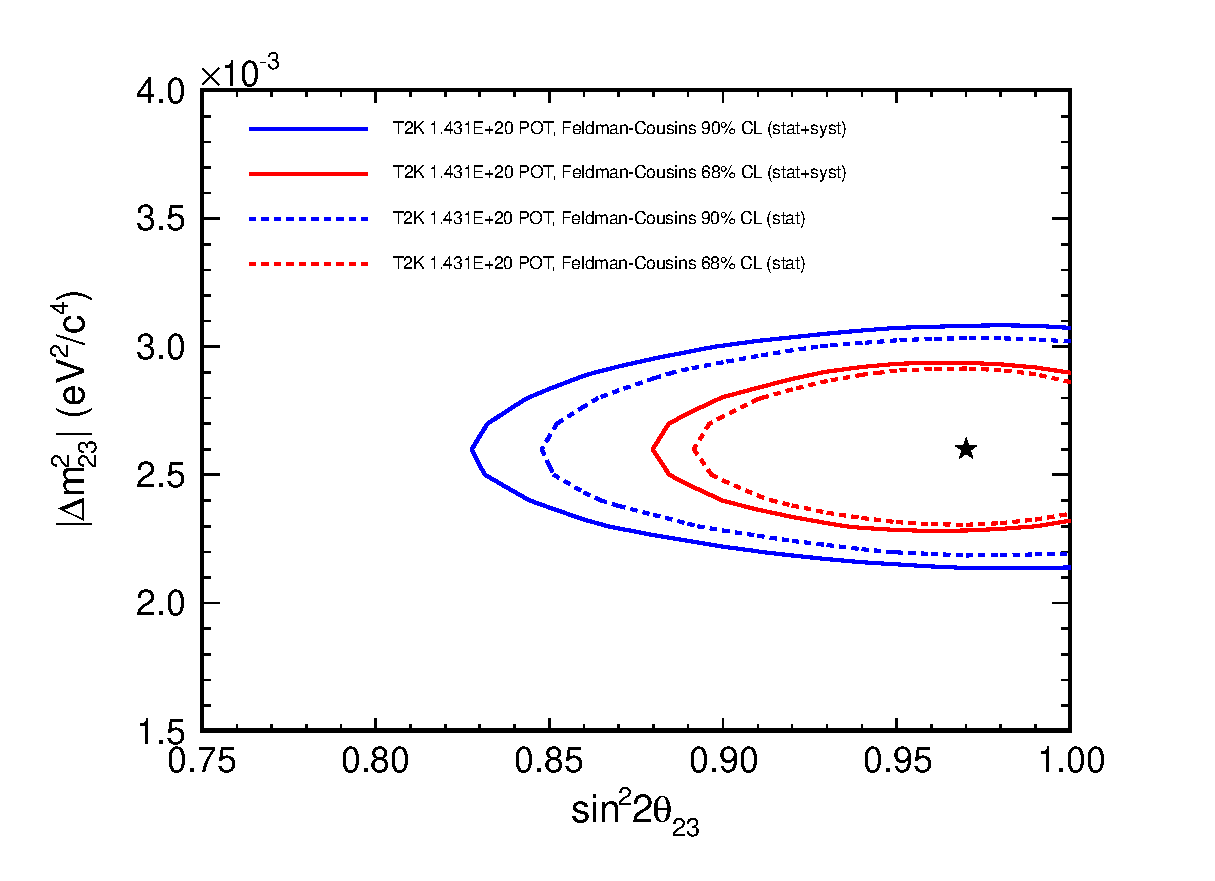
\includegraphics[width=30pc]{./images/confidence_regions/contour_run1p2_statsyst_genie.eps}
\caption{
  68\% and 90\% Feldman-Cousins confidence regions, with and without systematics,
  for the GENIE 2-flavour $\nu_{\mu}$-disappearance fit to the combined Run1+2 dataset
}
\label{fig:contour_run1p2_statsyst_genie}
\end{figure*}


\begin{figure*}[htb]
\center
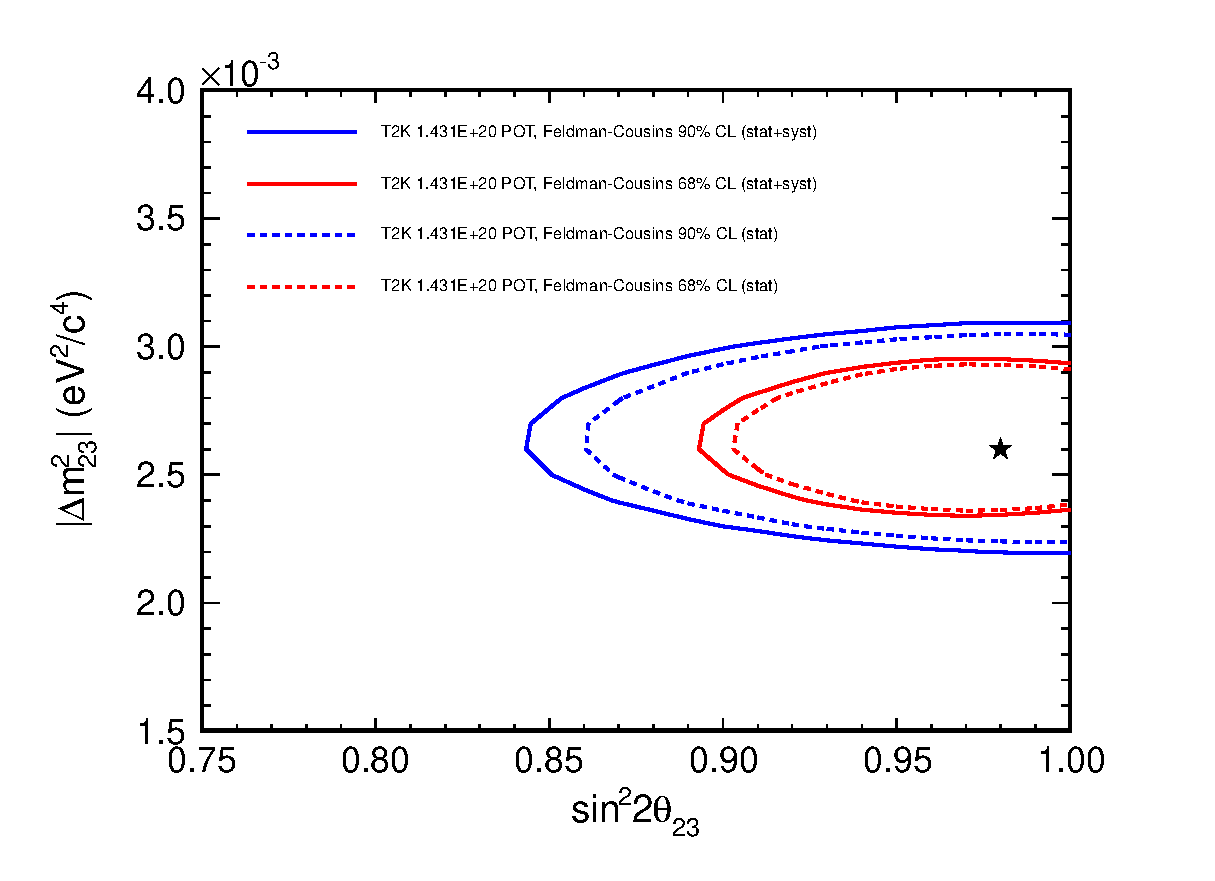
\includegraphics[width=30pc]{./images/confidence_regions/contour_run1p2_statsyst_neut.eps}
\caption{
  68\% and 90\% Feldman-Cousins confidence regions, with and without systematics,
  for the NEUT 2-flavour $\nu_{\mu}$-disappearance fit to the combined Run1+2 dataset
}
\label{fig:contour_run1p2_statsyst_neut}
\end{figure*}

%
% confidence regions for the Run1+2 fit - comparison with MINOS/K2K/SK-atm
%

\begin{figure*}[htb]
\center
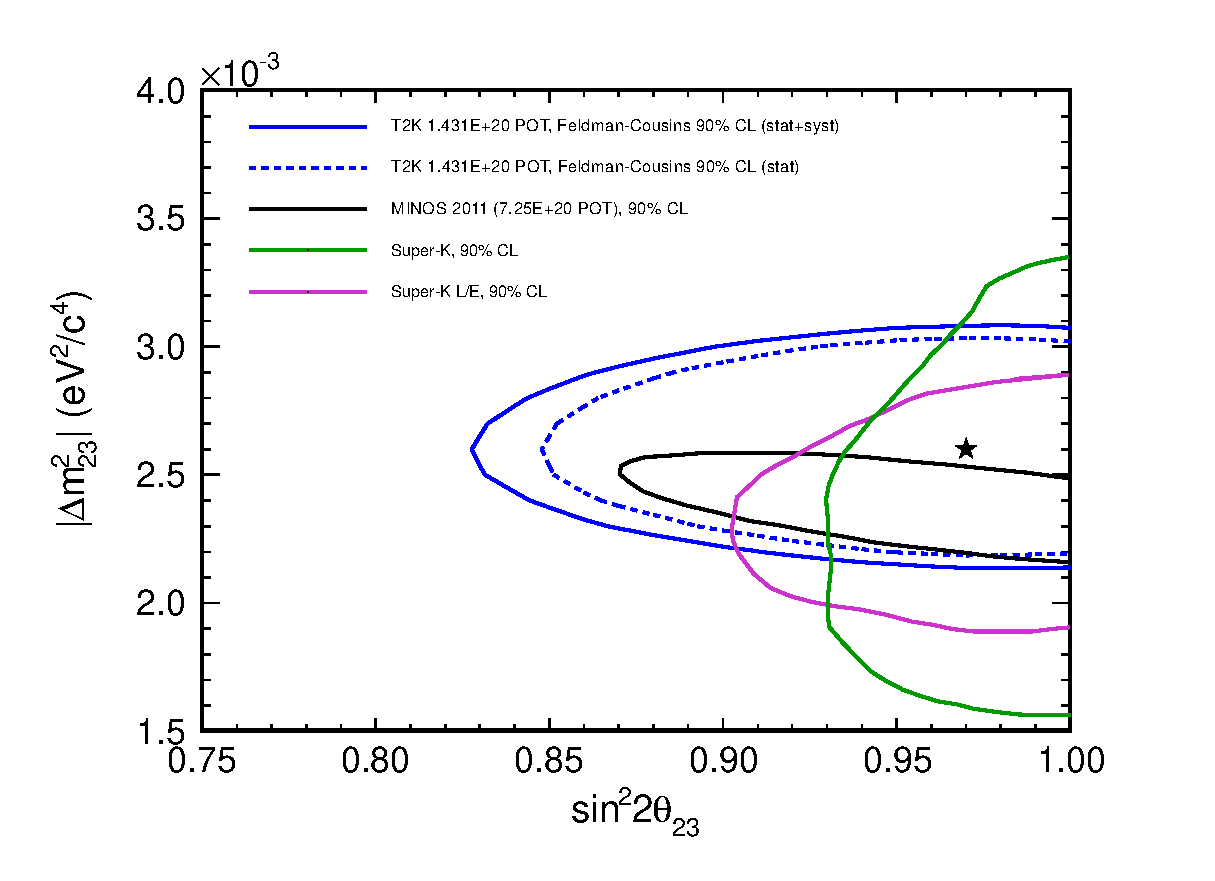
\includegraphics[width=30pc]{./images/confidence_regions/contour_run1p2_statsyst_genie_external_90clonly.eps}
\caption{
  90\% Feldman-Cousins confidence regions, with and without systematics,
  for the GENIE 2-flavour $\nu_{\mu}$-disappearance fit to the combined Run1+2 dataset:
  comparisons with results from MINOS and SuperK
}
\label{fig:contour_run1p2_statsyst_genie_external_90cl}
\end{figure*}

\begin{figure*}[htb]
\center
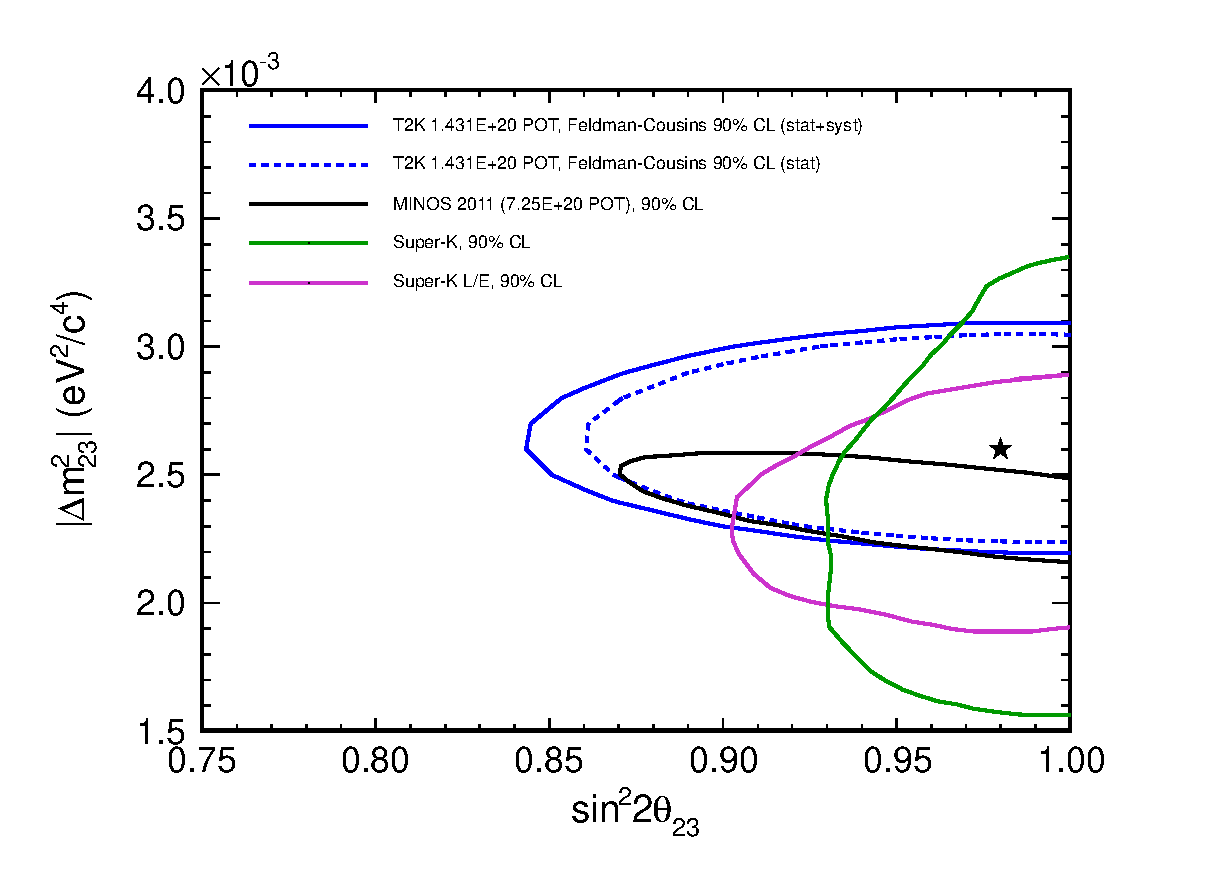
\includegraphics[width=30pc]{./images/confidence_regions/contour_run1p2_statsyst_neut_external_90clonly.eps}
\caption{
  90\% Feldman-Cousins confidence regions, with and without systematics,
  for the NEUT 2-flavour $\nu_{\mu}$-disappearance fit to the combined Run1+2 dataset:
  comparisons with results from MINOS and SuperK
}
\label{fig:contour_run1p2_statsyst_neut_external_90cl}
\end{figure*}


%
% confidence regions for the Run1+2 fit - comparison with MINOS/K2K/SK-atm
%

\begin{figure*}[htb]
\center
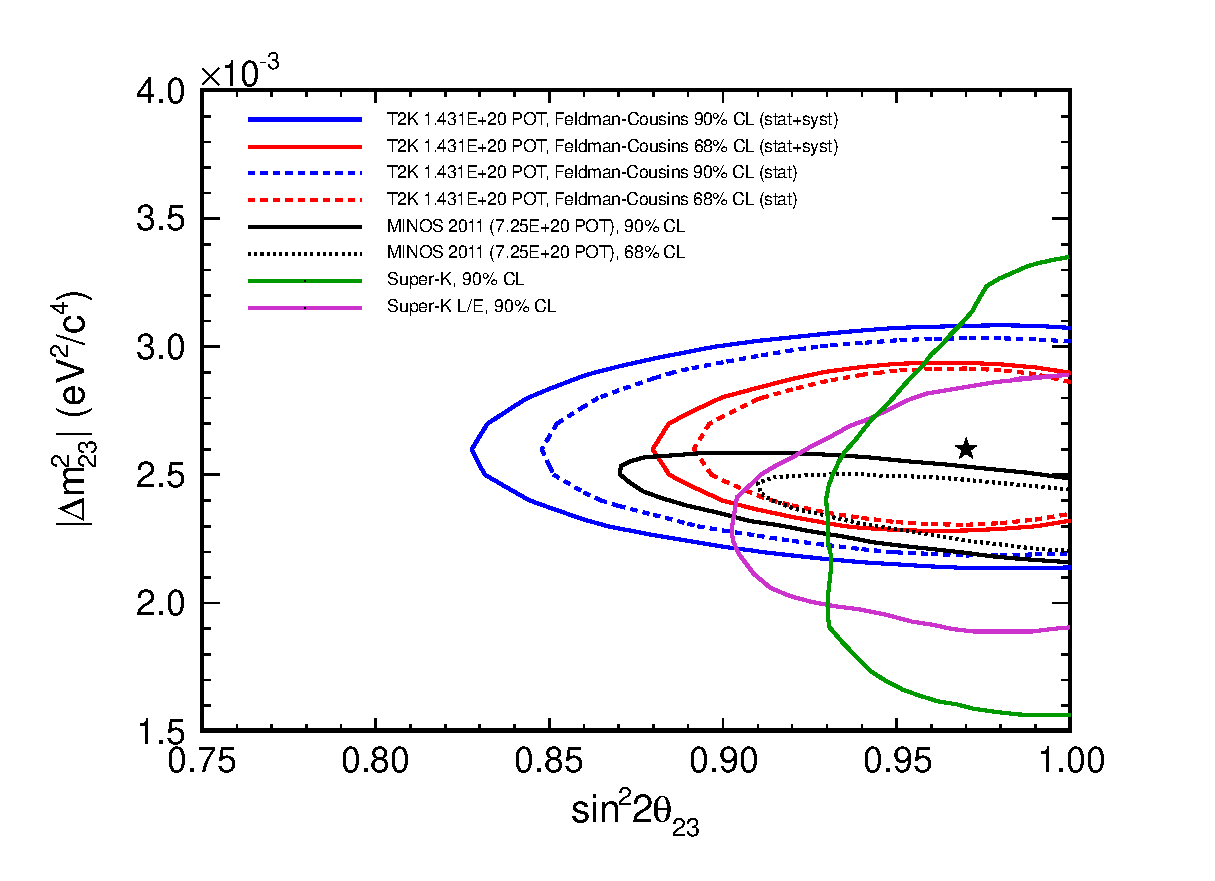
\includegraphics[width=30pc]{./images/confidence_regions/contour_run1p2_statsyst_genie_external.eps}
\caption{
  68\% and 90\% Feldman-Cousins confidence regions, with and without systematics,
  for the GENIE 2-flavour $\nu_{\mu}$-disappearance fit to the combined Run1+2 dataset:
  comparisons with MINOS 2011 68\% and 90\% contours and SuperK 90\% contour
}
\label{fig:contour_run1p2_statsyst_genie_external}
\end{figure*}

\begin{figure*}[htb]
\center
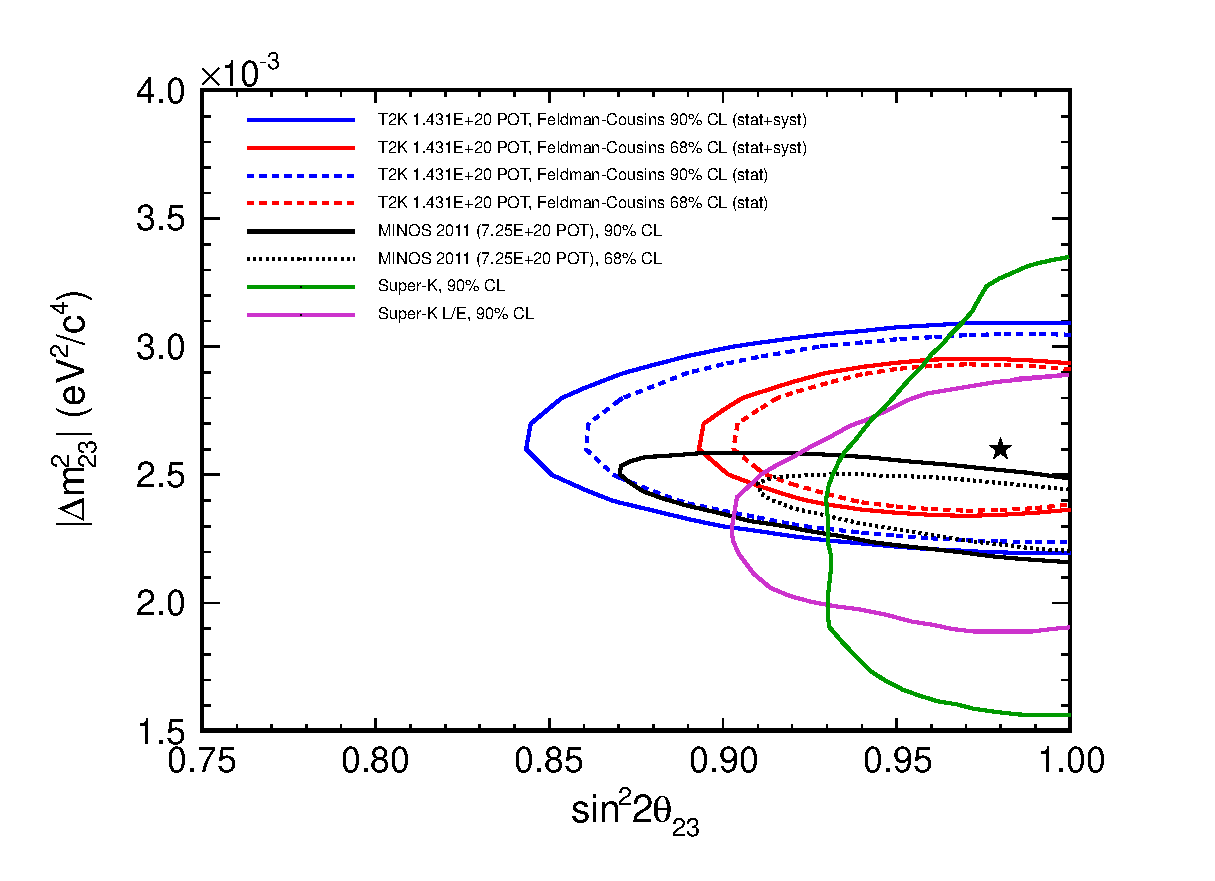
\includegraphics[width=30pc]{./images/confidence_regions/contour_run1p2_statsyst_neut_external.eps}
\caption{
  68\% and 90\% Feldman-Cousins confidence regions, with and without systematics,
  for the NEUT 2-flavour $\nu_{\mu}$-disappearance fit to the combined Run1+2 dataset:
  comparisons with MINOS 2011 68\% and 90\% contours and SuperK 90\%contour
}
\label{fig:contour_run1p2_statsyst_neut_external}
\end{figure*}


%
% confidence regions for the Run1+2 fit - comparison with sensitivity for MINOS-2011 params
%

\begin{figure*}[htb]
\center
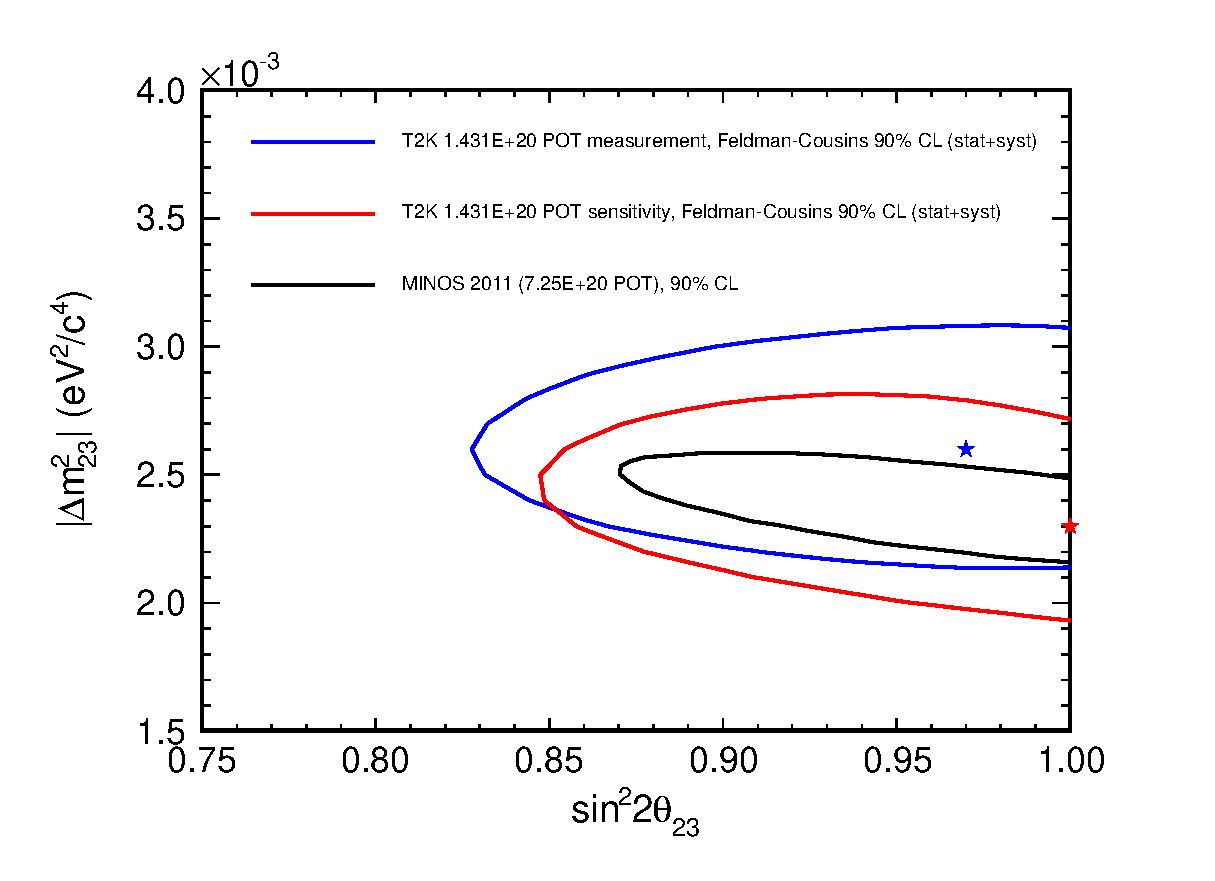
\includegraphics[width=30pc]{./images/confidence_regions/contour_run1p2_statsyst_genie_minos11sens.eps}
\caption{
  90\% Feldman-Cousins confidence regions (with systematics)
  for the GENIE 2-flavour $\nu_{\mu}$-disappearance fit to the combined Run1+2 dataset:
  comparisons with T2K 1.431$\times$10$^{20}$ POT sensitivity for $\nu_{\mu}$-disappearance with the MINOS 2011 
  best-fit values ($sin^{2}2\theta_{23}$ = 1.0 and $|\Delta m^{2}_{23}|$ = 2.32$\times10^{-3}$ $eV^{2}/c^{4}$).
  The MINOS 2011 90\% confidence region is also shown.
}
\label{fig:contour_run1p2_statsyst_genie_minos11sens}
\end{figure*}

\begin{figure*}[htb]
\center
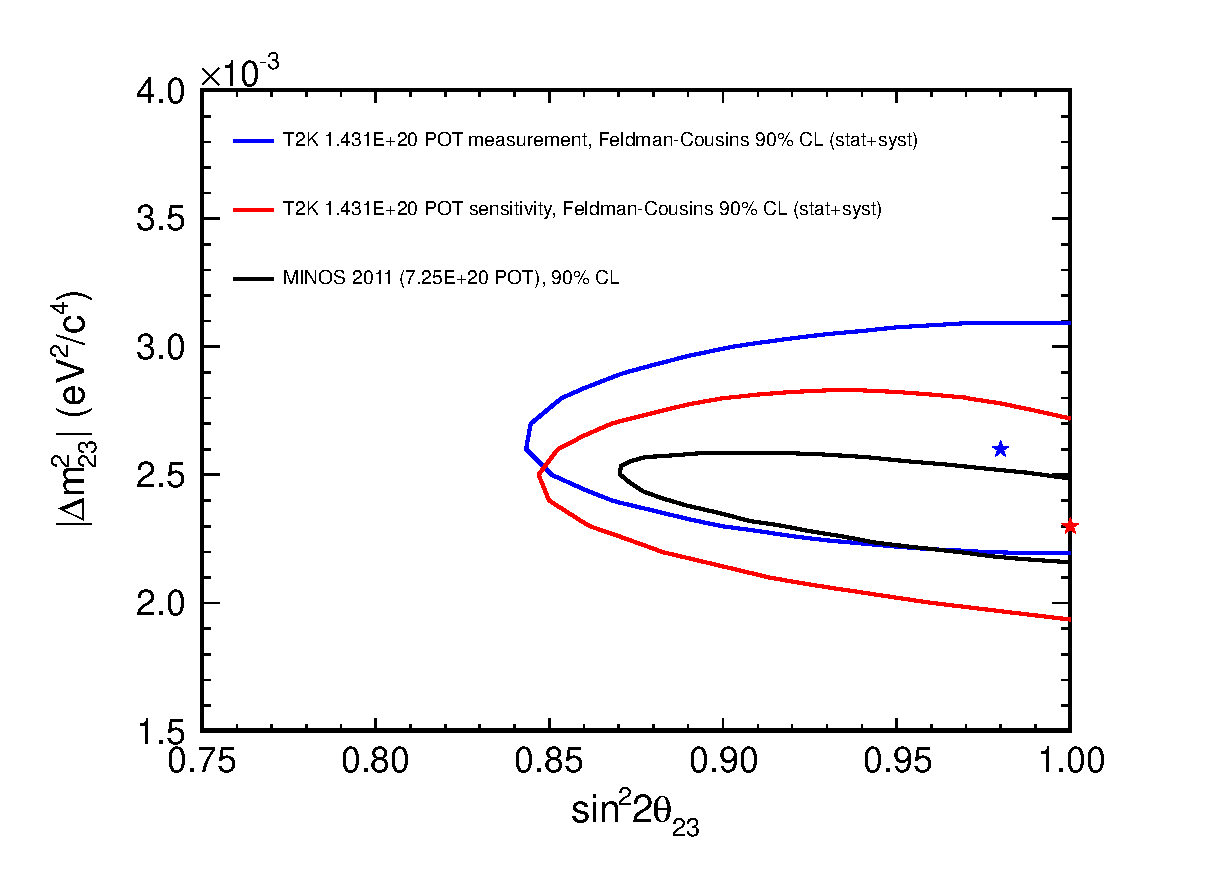
\includegraphics[width=30pc]{./images/confidence_regions/contour_run1p2_statsyst_neut_minos11sens.eps}
\caption{
  90\% Feldman-Cousins confidence regions (with systematics)
  for the NEUT 2-flavour $\nu_{\mu}$-disappearance fit to the combined Run1+2 dataset:
  comparisons with T2K 1.431$\times$10$^{20}$ POT sensitivity for $\nu_{\mu}$-disappearance with the MINOS 2011 
  best-fit values ($sin^{2}2\theta_{23}$ = 1.0 and $|\Delta m^{2}_{23}|$ = 2.32$\times10^{-3}$ $eV^{2}/c^{4}$).
  The MINOS 2011 90\% confidence region is also shown.
}
\label{fig:contour_run1p2_statsyst_neut_minos11sens}
\end{figure*}



%
% confidence regions for the Run1, Run2 and Run1+2 fits
%

\begin{figure*}[htb]
\center
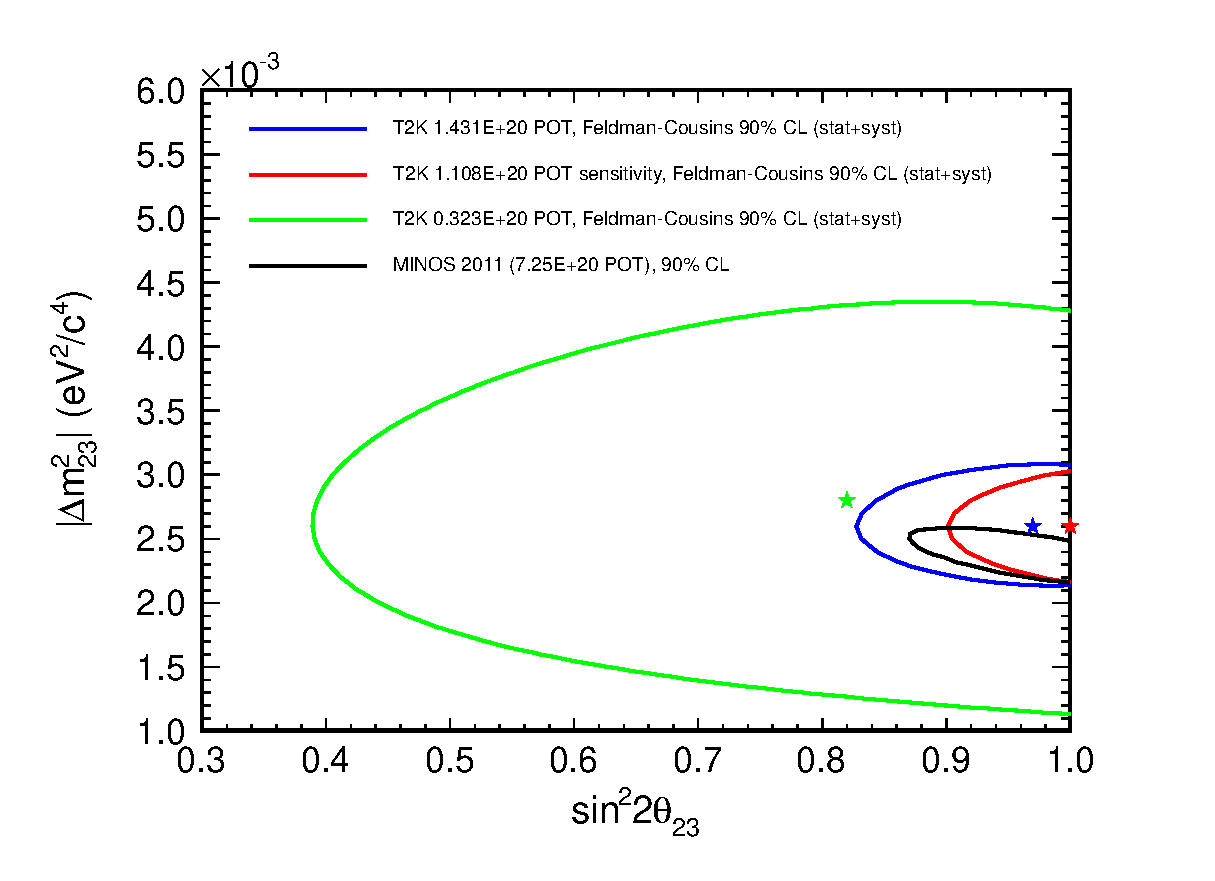
\includegraphics[width=30pc]{./images/confidence_regions/contour_statsyst_genie_3datasets.eps}
\caption{
  90\% Feldman-Cousins confidence regions (with systematics)
  for the GENIE 2-flavour $\nu_{\mu}$-disappearance fits to the Run1, Run2 and the combined Run1+2 datasets.
  The MINOS 2011 result is also shown for reference.
}
\label{fig:contour_statsyst_genie_3datasets}
\end{figure*}

\begin{figure*}[htb]
\center
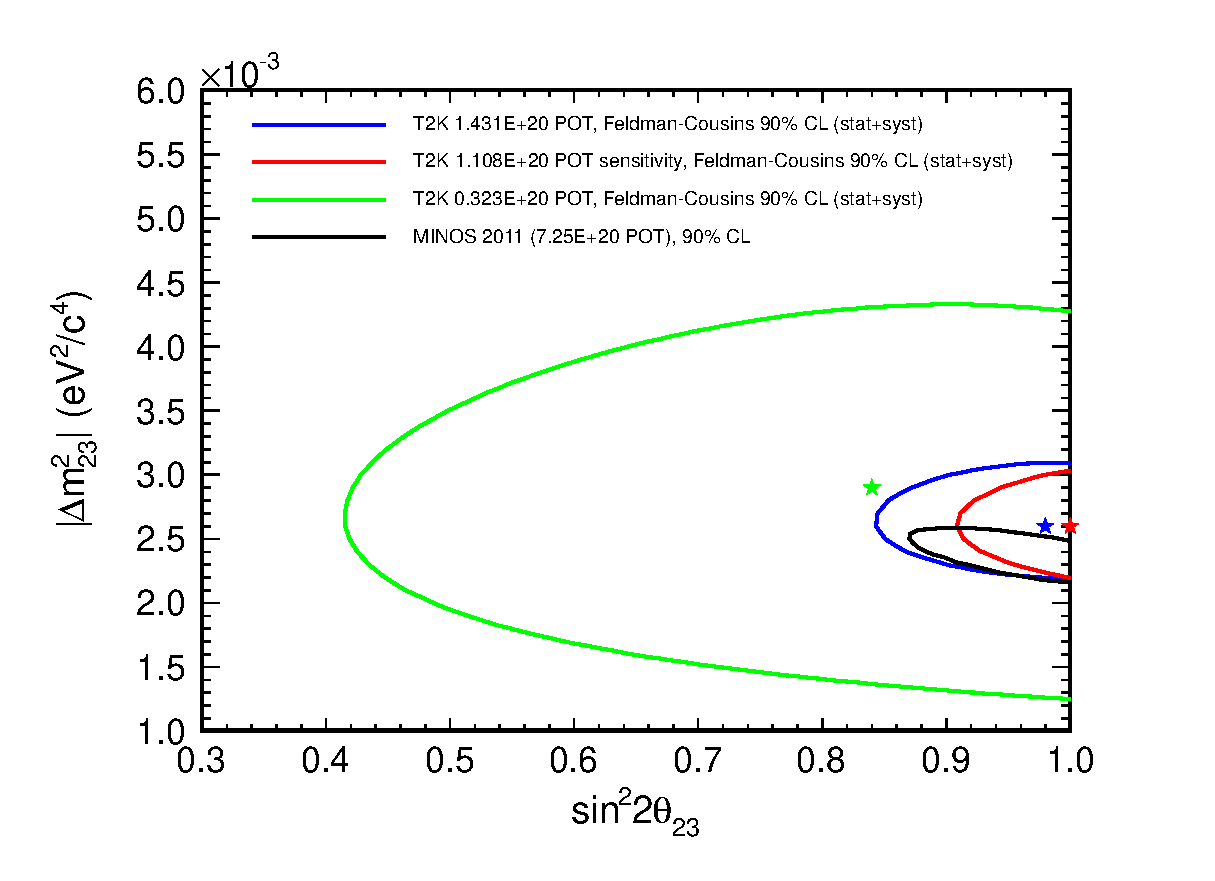
\includegraphics[width=30pc]{./images/confidence_regions/contour_statsyst_neut_3datasets.eps}
\caption{
  90\% Feldman-Cousins confidence regions (with systematics)
  for the NEUT 2-flavour $\nu_{\mu}$-disappearance fits to the Run1, Run2 and the combined Run1+2 datasets.
  The MINOS 2011 result is also shown for reference.
}
\label{fig:contour_statsyst_neut_3datasets}
\end{figure*}

